\section{Eldrid}\label{eldrid}

Tags: Città Creatore: Lorenzo Luogo: Mitegard Meridionale, Valtara

\section{Eldrid}\label{eldrid-1}

\begin{center}\rule{0.5\linewidth}{0.5pt}\end{center}

\begin{figure}
\centering
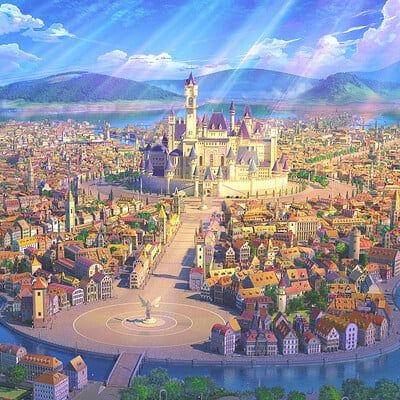
\includegraphics{eldrid.jpg}
\caption{eldrid.jpg}
\end{figure}

Informazioni Generali

Tipo di Luogo: Città Stato

Dimensioni:

Altitudine: 0 m slm

Popolazione: 150 000 abitanti

Paese: Terre Libere di Valtara

Luogo: Mitegard Meridionale, Valtara

\begin{center}\rule{0.5\linewidth}{0.5pt}\end{center}

\subsection{1. Descrizione Generale}\label{descrizione-generale}

\begin{center}\rule{0.5\linewidth}{0.5pt}\end{center}

Eldrid è una maestosa città situata nella regione del Mitegard
Meridionale, nella Valtara settentrionale. La città riveste
un'importanza straordinaria all'interno della regione, essendo una delle
quattro città-stato di Valtara. La sua influenza si estende ampiamente
sul territorio circostante, e grazie alla sua posizione privilegiata sul
Mare di Smeraldo, è uno dei porti più vitali e fiorenti, seconda
solamente alla città-stato di Azura. La città sorge alla foce del fiume
Eldrio e si estende in una cornice mozzafiato tra il mare e le colline
circostanti.

\subsection{2. Storia}\label{storia}

\begin{center}\rule{0.5\linewidth}{0.5pt}\end{center}

Eldrid ha sempre giocato un ruolo centrale nell'economia e nella
politica della regione. Con il passare dei secoli, la città ha
prosperato sotto il dominio di varie potenze che hanno riconosciuto la
sua importanza strategica, contribuendo a consolidare la sua posizione
come snodo vitale nel commercio via mare e via terra. La città ha avuto
un ruolo chiave nel periodo dei Comuni, essendo la prima città di
Valtara a dichiarare la propria indipendenza, con l'
\href{Editto\%20di\%20Eldrid\%20fc90df43131849e391648cf2cbc2d5b1.md}{Editto
di Eldrid} . Questo atto di audacia ha gettato le basi per la creazione
delle Terre Libere di Valtara, unendo popolazioni provenienti da diverse
terre sotto un unico stendardo di libertà e autogoverno. In precedenza,
Eldrid faceva parte di un regno vassallo, ormai decaduto, dell'Impero di
Disharta. Oggi, la città si presenta come una repubblica vibrante e
fiorente.

\subsection{3. Geografia}\label{geografia}

\begin{center}\rule{0.5\linewidth}{0.5pt}\end{center}

Eldrid sorge all'incrontro tra il fiume Eldrio e il Mare di Smeraldo.
Questa posizione ne fa uno dei principali centri commerciali e portuali
della regione. Le acque calme del mare offrono un sicuro rifugio alle
navi mercantili, mentre le colline circostanti regalano uno scenario
pittoresco e un ambiente protetto. La città è nota per il suo imponente
faro, visibile da chilometri di distanza e fondamentale per i
navigatori.

\begin{figure}
\centering
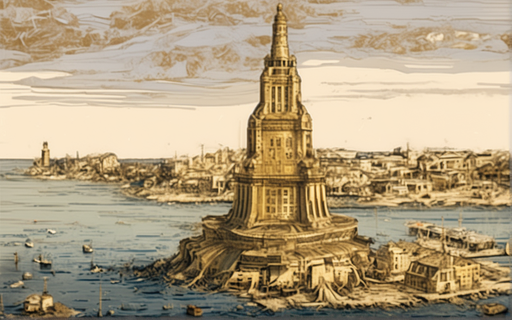
\includegraphics{faro-haze-ultra-detailed-film-photography-light-leaks-larry-bud-melman-trending-on-artstation.png}
\caption{Antica litografia che ritrae il faro di Eldrid}
\end{figure}

Antica litografia che ritrae il faro di Eldrid

\subsection{4. Economia}\label{economia}

\begin{center}\rule{0.5\linewidth}{0.5pt}\end{center}

L'economia di Eldrid è fortemente incentrata sul commercio e sui
trasporti marittimi. La città serve da fulcro per l'importazione e
l'esportazione di merci, giocando un ruolo fondamentale nell'economia
regionale. Il porto di Eldrid è un importante centro di scambio di merci
provenienti da tutte le Terre Libere di Valtara e da tutto il
continente, consolidando così la posizione predominante della città nel
panorama economico della regione.

\subsection{5. Demografia}\label{demografia}

\begin{center}\rule{0.5\linewidth}{0.5pt}\end{center}

Eldrid vanta una popolazione eclettica e multietnica di 150.000
abitanti, giunti da ogni angolo di Valtara e oltre. Le strade della
città sono animate da individui di diverse razze e culture, creando una
vivace atmosfera di scambio e collaborazione. La sua popolazione
eterogenea è un testimone della ricca storia e del ruolo centrale di
Eldrid nell'evoluzione delle Terre Libere di Valtara. La città ha
assistito a un notevole aumento demografico negli ultimi cinquant'anni,
un periodo in cui la maggior parte dei residenti delle valli circostanti
hanno abbandonato le loro terre d'origine per trasferirsi nella città in
cerca di opportunità economiche e sociali. Questo flusso migratorio ha
portato a un rapido accrescimento della popolazione urbana, dando luogo
a una vivace espansione edilizia e commerciale che ha superato i confini
cittadini. Tuttavia, questo aumento ha comportato uno spopolamento
significativo della regione circostante, generando uno squilibrio
demografico che ha suscitato preoccupazioni per il futuro equilibrio
ambientale e sociale della zona. L'amministrazione cittadina sta
attuando misure mirate per mitigare tale squilibrio, promuovendo un uso
sostenibile delle risorse e incoraggiando la riqualificazione delle zone
circostanti per attrarre nuovamente la popolazione e ridistribuire in
modo più equo il tessuto sociale e demografico della regione.

\subsection{6. Cultura}\label{cultura}

La cultura di Eldrid riflette la diversità delle sue genti e l'apertura
verso nuove idee e tradizioni. La città è rinomata per le sue
celebrazioni animate, le arti affascinanti e la cucina variegata. Ogni
anno, le strade si animano con feste e parate colorate, mentre teatri,
gallerie d'arte e mercati tradizionali contribuiscono a creare
un'atmosfera culturale vivace e coinvolgente.

\subsection{7. Governo}\label{governo}

\begin{center}\rule{0.5\linewidth}{0.5pt}\end{center}

Eldrid è governata da un sistema repubblicano unico, che si distingue
per la sua struttura innovativa e per l'equilibrio tra stabilità e
dinamismo. I rappresentanti sono eletti ogni sette anni tramite un
processo elettorale rigoroso e trasparente, che coinvolge attivamente la
popolazione e incoraggia la partecipazione democratica. La città elegge
75 rappresentanti che formeranno il nucleo del Parlamento, il cui ruolo
è fondamentale nel processo decisionale della città. Il Parlamento
lavora attivamente con il Console, la figura centrale del governo. Il
Console è un capo di stato scelto direttamente dai rappresentanti eletti
ed è una figura di grande prestigio e autorità, detiene una vasta gamma
di poteri che gli consentono di dirigere gli affari interni ed esterni
della città. Il mandato del Console ha una durata di un anno e non è
rieleggibile nel corso dei sette anni di governo, garantendo così una
rotazione regolare e l'opportunità di rinnovamento all'interno della
leadership cittadina. Ogni governo, quindi, eleggerà sette consoli,
ciascuno con la responsabilità di guidare la città in base ai principi
di giustizia, equità e progresso sociale.
